% You should title the file with a .tex extension (hw1.tex, for example)
\documentclass[a4paper, 11pt]{article}

\usepackage{amsmath}
\usepackage{amssymb}
\usepackage{fancyhdr}
\usepackage{graphicx}

\usepackage[margin=1in]{geometry}

\newcommand{\question}[2] {\vspace{.25in} \hrule\vspace{0.5em}
\noindent{\bf #1: #2} \vspace{0.5em}
\hrule \vspace{.10in}}
\renewcommand{\part}[1] {\vspace{.10in} {\bf (#1)}}

\newcommand{\myname}{Natthakan Euaumpon}
\newcommand{\myemail}{natthakaneuaumpon@gmail.com}
\newcommand{\myhwnum}{Report}

\setlength{\parindent}{0pt}
\setlength{\parskip}{5pt plus 1pt}
 
\pagestyle{fancyplain}
\lhead{\fancyplain{}{\textbf{\myhwnum}}}      % Note the different brackets!
\rhead{\fancyplain{}{\myname\\ \myemail}}
\chead{\fancyplain{}{ICCS222 }}

\begin{document}

\medskip                        % Skip a "medium" amount of space
                                % (latex determines what medium is)
                                % Also try: \bigskip, \littleskip

\thispagestyle{plain}
\begin{center}                  % Center the following lines
{\Large ICCS222:  \myhwnum} \\
\myname \\
\myemail \\
April 2020 \\
\end{center}
\question{1}{purpose}
The purpose of this experiment is to find the differences in trends for 3 different page replacement algorithm on 3 difference trace files and the differences in total page faults between 256 and 1024 bits of page size. This is to find out is there an algorithm that works better than the others on each trace files.\\
To run the file we need to run 3 commands:
\begin{enumerate}
	\item gcc -o virtmem virtmem.c
	\item chmod +x run.sh
	\item \textbackslash run.sh
\end{enumerate}
\question{2}{graph}
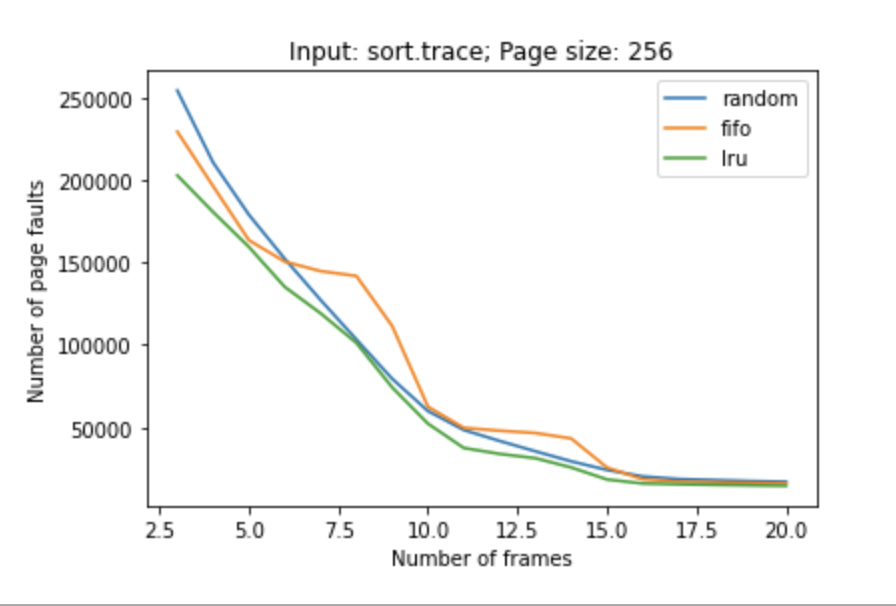
\includegraphics[width=\textwidth]{sortTrace256.png}\\
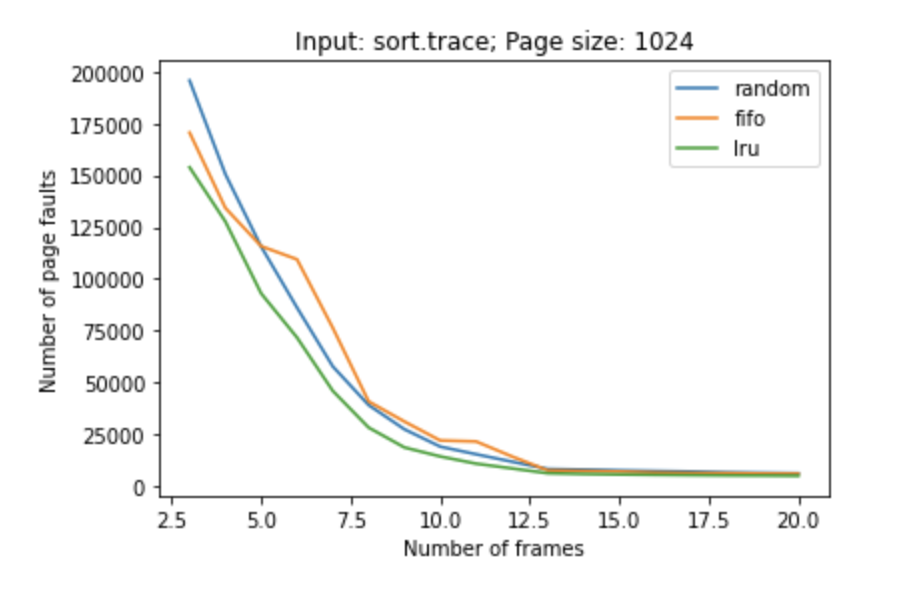
\includegraphics[width=\textwidth]{sortTrace1024.png}\\
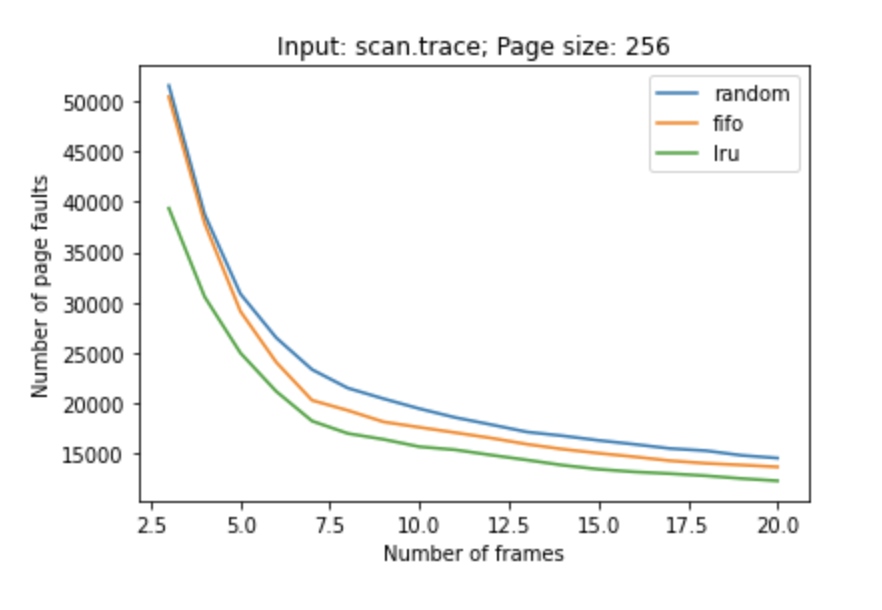
\includegraphics[width=\textwidth]{scanTrace256.png}\\
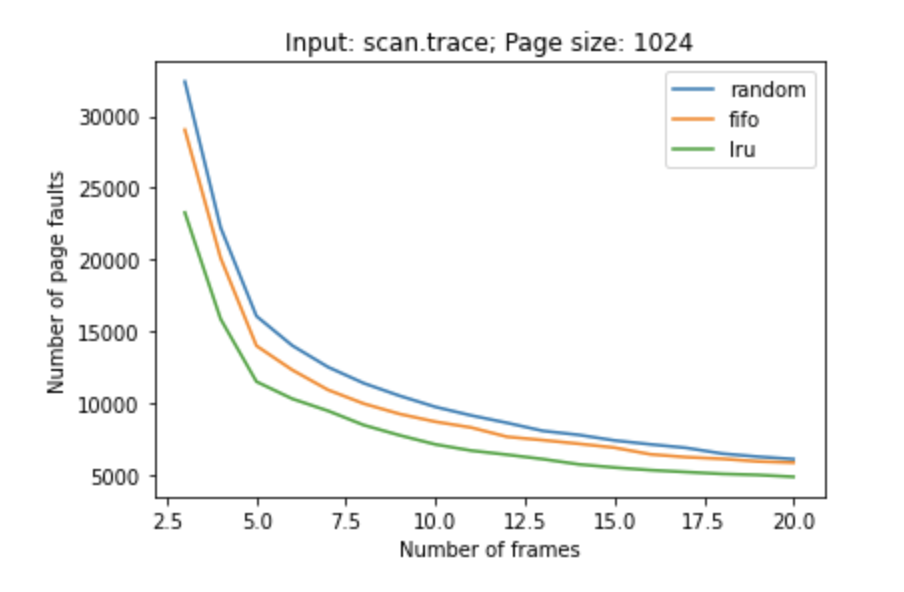
\includegraphics[width=\textwidth]{scanTrace1024.png}\\
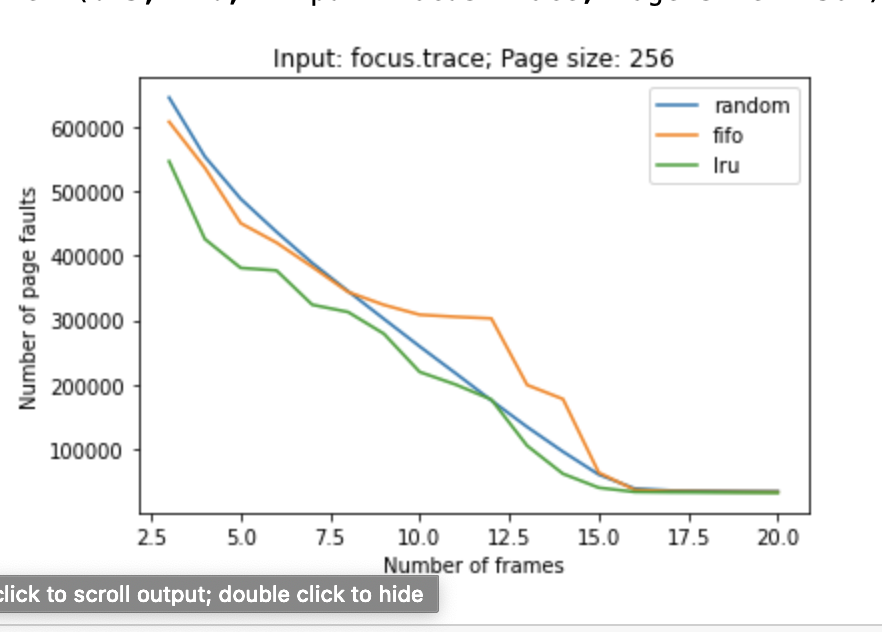
\includegraphics[width=\textwidth]{focusTrace256.png}\\
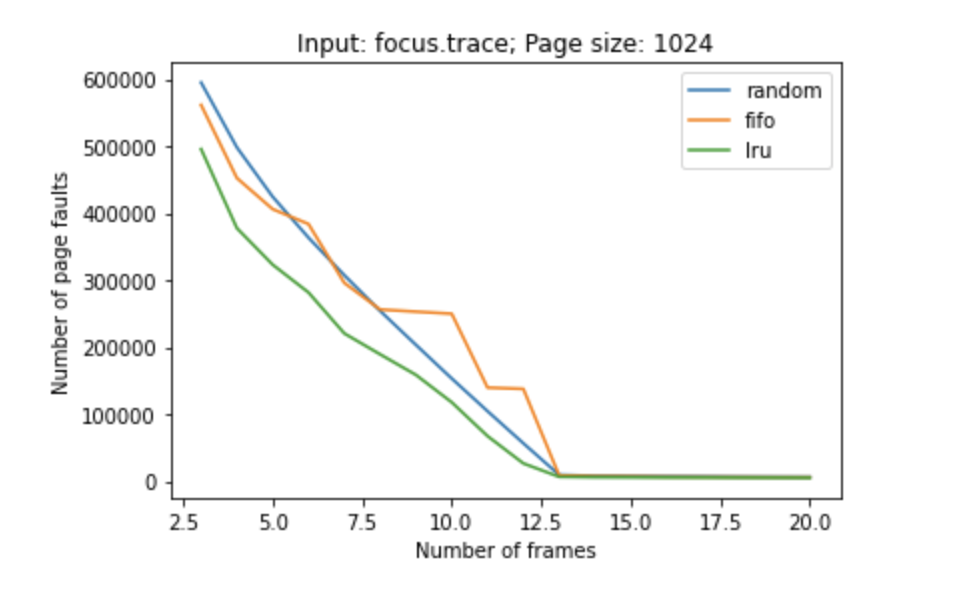
\includegraphics[width=\textwidth]{focusTrace1024.png}
\question{3}{Trends}
\begin{enumerate}
	\item sort.trace\\
	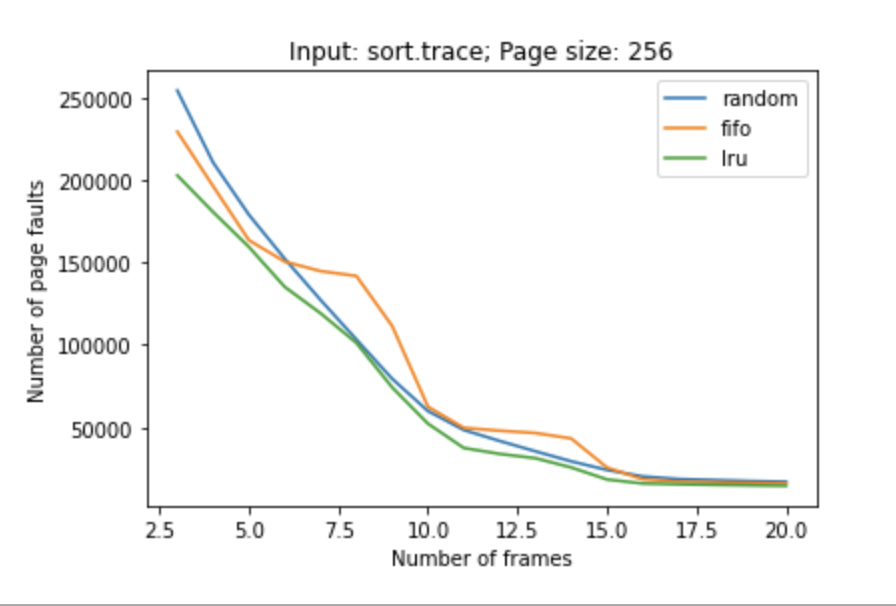
\includegraphics[width=\textwidth]{sortTrace256.png}\\
	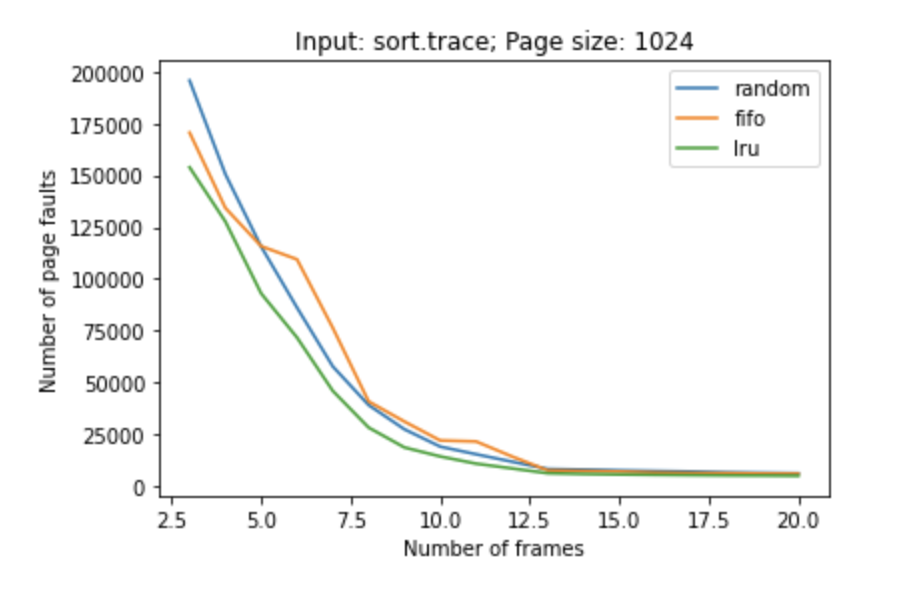
\includegraphics[width=\textwidth]{sortTrace1024.png}\\
	From this 2 graphs we can easily indicate that lru performs the best for both 256 and 1024 page size. As the total page faults per frame is the lowest compare to the other method.
	\item scan.trace\\
	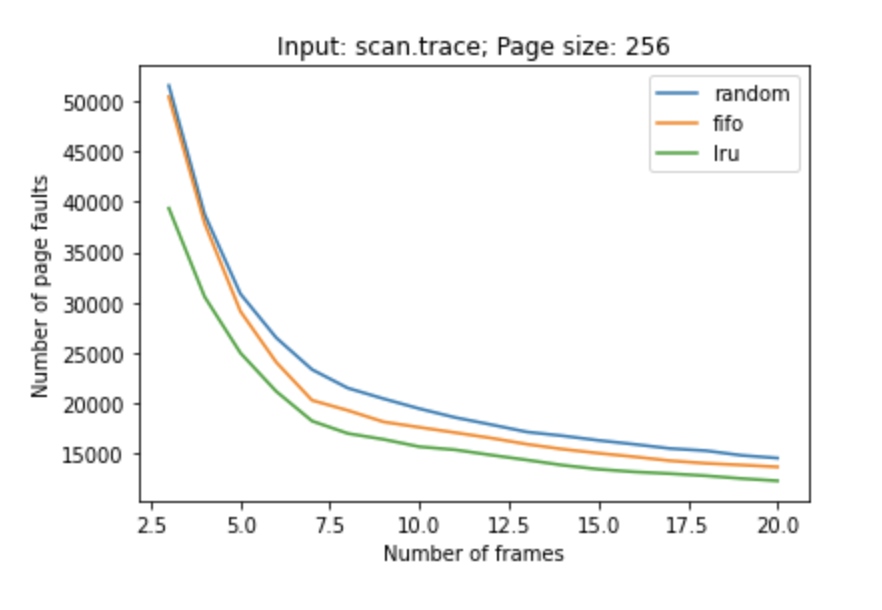
\includegraphics[width=\textwidth]{scanTrace256.png}\\
	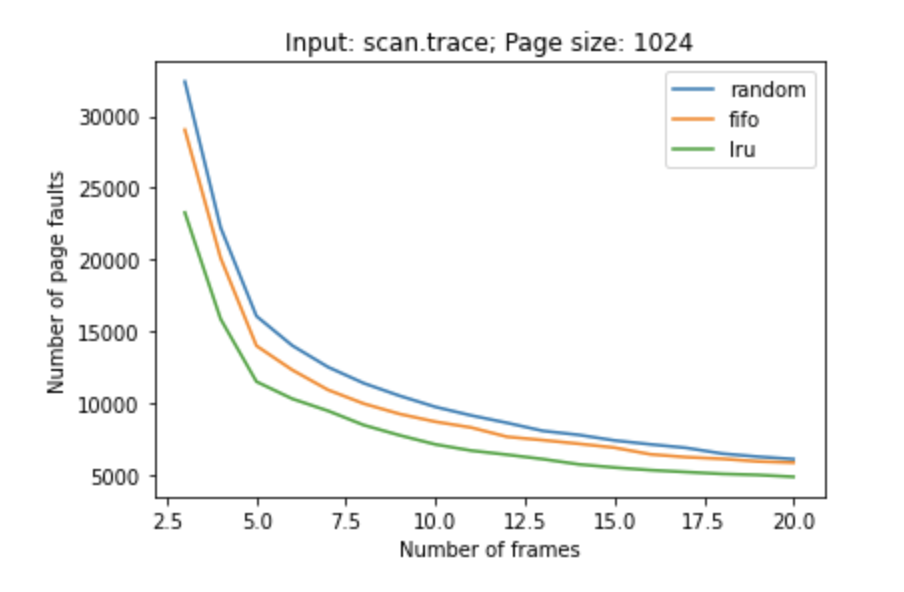
\includegraphics[width=\textwidth]{scanTrace1024.png}\\
	For this trace files Iru also works the best according to the graph it has the least number of page faults compare to the other 2.
	\item focus.trace\\
	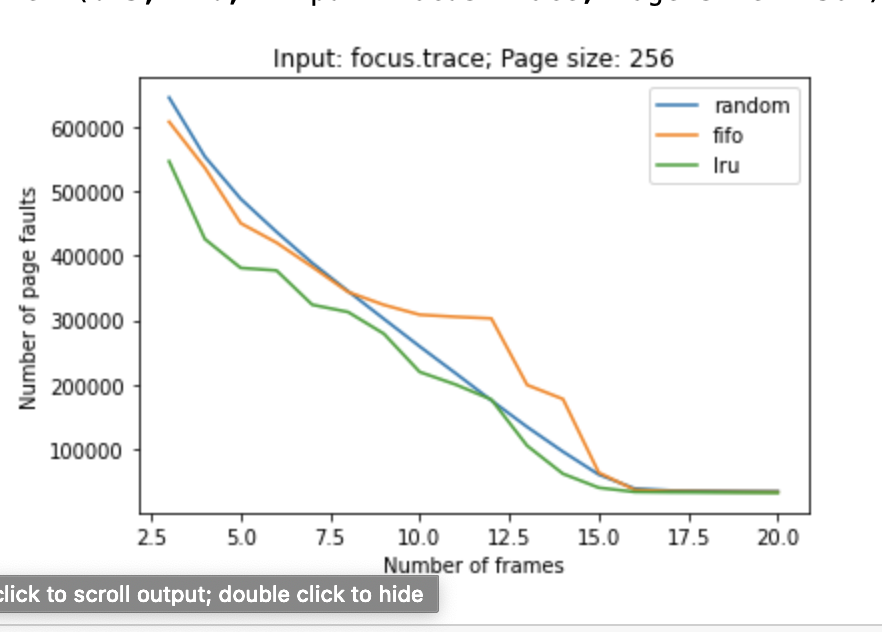
\includegraphics[width=\textwidth]{focusTrace256.png}\\
	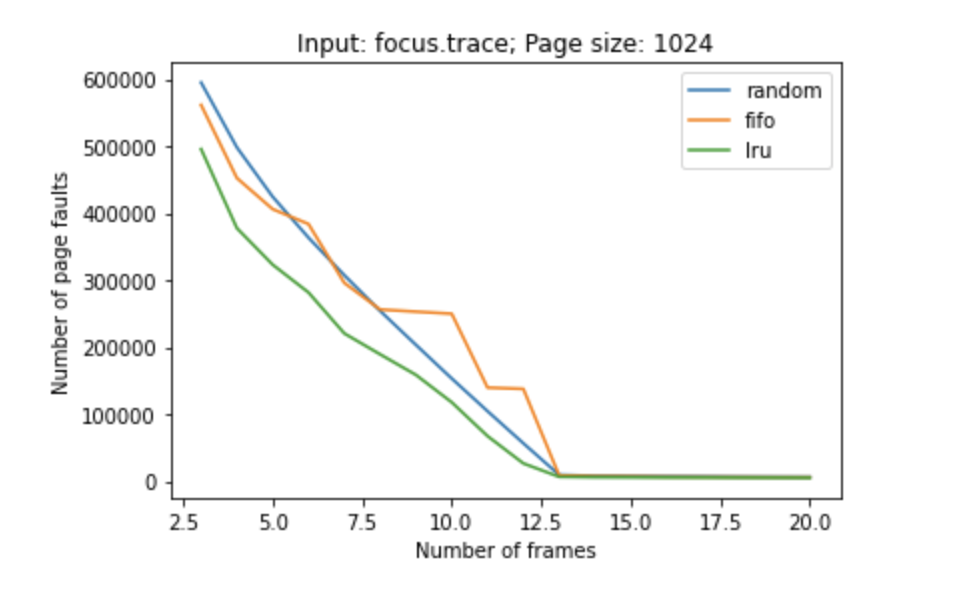
\includegraphics[width=\textwidth]{focusTrace1024.png}\\
	For this trace files Iru also works the best accord tp the graph. Eventhogh the graph is fructuated at the lower number of frames. 
\end{enumerate}
\end{document}

